% ---------------------------------------------------------------------------
% Preamble requirements:
%   \usepackage{tikz}            % NO \usetikzlibrary needed
%   \usepackage[ruled,vlined,linesnumbered]{algorithm2e}   % NOT with {algorithm}
%   \usepackage{float}                                     % algorithm [H]
%   \usepackage{amsmath,amssymb,graphicx}
% NOTE 1: the tikz style is called `outbox', not `out' -- `out' is a built-in
%   tikz key (to[out=..,in=..]) and shadowing it makes \node[out] a hard error.
% NOTE 2: uses no tikz libraries and no `diamond' shape, so it cannot fail on a
%   missing \usetikzlibrary{shapes.geometric}.
% NOTE 3: algorithm2e's [H] is illegal in twocolumn mode, and algorithm2e must
%   NOT be loaded alongside {algorithm}.  {algpseudocode} alongside is fine.
% ---------------------------------------------------------------------------
\begin{figure*}[t]
\centering
% ---------- (a) the pipeline ----------
\resizebox{\textwidth}{!}{%
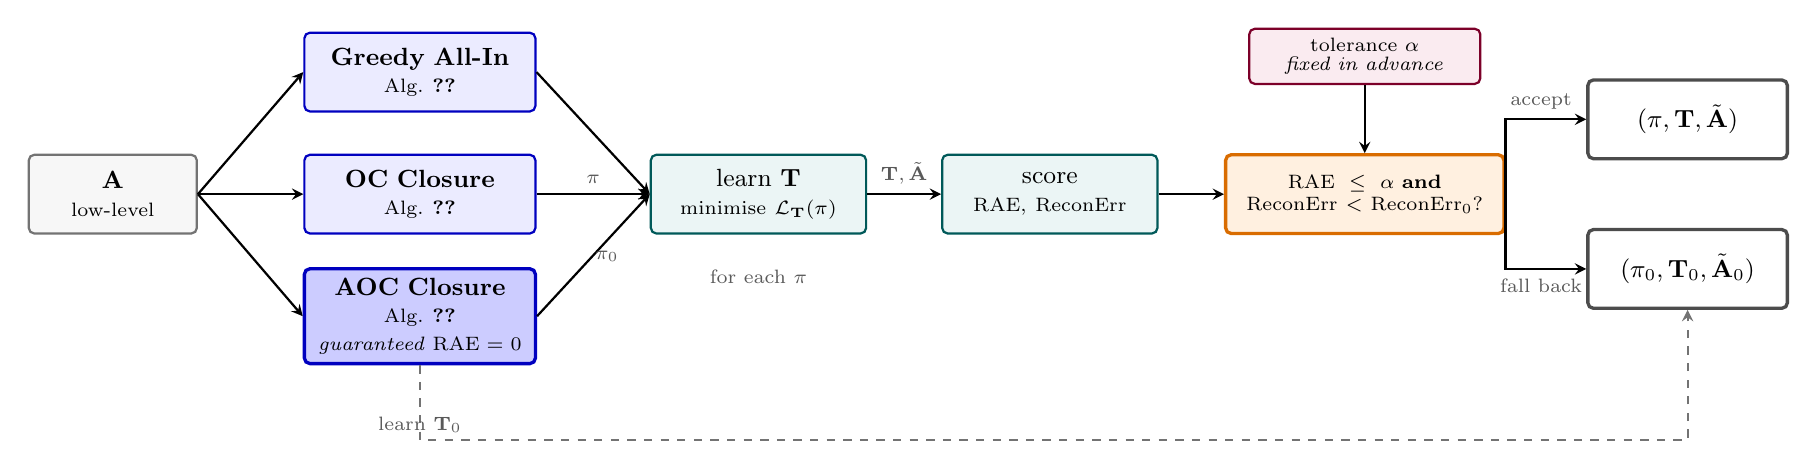
\begin{tikzpicture}[
    >=stealth, node distance=0pt,
    stage/.style={rounded corners=2pt, draw=black!55, fill=black!3, thick,
                  minimum height=1.0cm, text width=1.9cm, align=center, font=\small},
    algbox/.style={rounded corners=2pt, draw=blue!75!black, fill=blue!8, thick,
                   minimum height=1.0cm, text width=2.7cm, align=center, font=\small},
    fbbox/.style={rounded corners=2pt, draw=blue!75!black, fill=blue!20, very thick,
                  minimum height=1.0cm, text width=2.7cm, align=center, font=\small},
    obj/.style={rounded corners=2pt, draw=teal!70!black, fill=teal!8, thick,
                minimum height=1.0cm, text width=2.5cm, align=center, font=\small},
    dial/.style={rounded corners=2pt, draw=purple!65!black, fill=purple!8, thick,
                 minimum height=0.7cm, text width=2.7cm, align=center, font=\scriptsize},
    gate/.style={rounded corners=2pt, draw=orange!85!black, fill=orange!12, very thick,
                 minimum height=1.0cm, text width=3.3cm, align=center, font=\scriptsize},
    outbox/.style={rounded corners=2pt, draw=black!70, fill=white, very thick,
                   minimum height=1.0cm, text width=2.3cm, align=center, font=\small},
    lbl/.style={font=\scriptsize, text=black!65, align=center}
]
\node[stage]  (A)   at (0,0)       {$\mathbf{A}$\\[-1pt]{\scriptsize low-level}};

% --- the three partition learners, run in parallel on the same A ---
\node[algbox] (ga)  at (3.9, 1.55) {\textbf{Greedy All-In}\\[-1pt]{\scriptsize Alg.~\ref{alg:greedy}}};
\node[algbox] (oc)  at (3.9, 0.00) {\textbf{OC Closure}\\[-1pt]{\scriptsize Alg.~\ref{alg:oc}}};
\node[fbbox]  (aoc) at (3.9,-1.55) {\textbf{AOC Closure}\\[-1pt]{\scriptsize Alg.~\ref{alg:aoc}}%
                                    \\[-1pt]{\scriptsize\itshape guaranteed $\mathrm{RAE}=0$}};

\node[obj]    (fit) at (8.2, 0)    {learn $\mathbf{T}$\\[-1pt]{\scriptsize minimise $\mathcal{L}_{\mathbf{T}}(\pi)$}};
\node[obj]    (sc)  at (11.9,0)    {score\\[-1pt]{\scriptsize $\mathrm{RAE}$, $\mathrm{ReconErr}$}};
\node[dial]   (al)  at (15.9,1.75) {tolerance $\alpha$\\[-1pt]\emph{fixed in advance}};
\node[gate]   (g)   at (15.9,0)    {$\mathrm{RAE}\leq\alpha$ \textbf{and}\\
                                    $\mathrm{ReconErr}<\mathrm{ReconErr}_{0}$?};
\node[outbox] (acc) at (20.0, 0.95){$(\pi,\mathbf{T},\tilde{\mathbf{A}})$};
\node[outbox] (fb)  at (20.0,-0.95){$(\pi_{0},\mathbf{T}_{0},\tilde{\mathbf{A}}_{0})$};

\draw[->,thick] (A.east) -- (ga.west);
\draw[->,thick] (A.east) -- (oc.west);
\draw[->,thick] (A.east) -- (aoc.west);
\draw[->,thick] (ga.east)  -- (fit.west);
\draw[->,thick] (oc.east)  -- node[lbl,above]{$\pi$} (fit.west);
\draw[->,thick] (aoc.east) -- node[lbl,below,pos=0.62]{$\pi_{0}$} (fit.west);
\draw[->,thick] (fit) -- node[lbl,above]{$\mathbf{T},\tilde{\mathbf{A}}$} (sc);
\draw[->,thick] (sc)  -- (g);
\draw[->,thick] (al)  -- (g);
\draw[->,thick] (g.east) |- (acc) node[lbl,above,pos=0.72]{accept};
\draw[->,thick] (g.east) |- (fb)  node[lbl,below,pos=0.72]{fall back};
% the fallback candidate is fitted from pi_0 and is always available
\draw[->,thick,dashed,black!55] (aoc.south) -- ++(0,-0.95)
      node[lbl,below,pos=0.55]{learn $\mathbf{T}_{0}$} -| (fb.south);
\node[lbl] at (8.2,-1.05) {for each $\pi$};
\end{tikzpicture}}

\vspace{0.5em}
% ---------- (b) the three partition learners ----------
\begin{minipage}[t]{0.32\textwidth}\vspace{0pt}
\begin{algorithm}[H]\footnotesize\hyphenpenalty=10000\exhyphenpenalty=10000
\SetAlgoLined\DontPrintSemicolon
\SetAlCapFnt{\scriptsize}\SetAlCapNameFnt{\scriptsize}
\SetKwFunction{Closure}{Closure}
\SetKwProg{Fn}{Function}{:}{}
\caption{OC Closure}\label{alg:oc}
\KwIn{$\mathbf{A}\in\mathbb{R}^{p\times p}$, draws $d$}
\KwOut{$\pi$: One-Child}
$\pi^{\star}\leftarrow\varnothing$;\ $\ell^{\star}\leftarrow\infty$\;
\For{$t=1,\dots,d$}{
  $\pi\leftarrow$ \Closure{$\mathbf{A}$}\;
  \If{$\mathrm{IL}(\pi)<\ell^{\star}$}{
    $\pi^{\star}\leftarrow\pi$;\ $\ell^{\star}\leftarrow\mathrm{IL}(\pi)$\;
  }
}
\Return $\pi^{\star}$\;
\BlankLine
\Fn{\Closure{$\mathbf{A}$}}{
  $\pi\leftarrow$ singletons\;
  \Repeat{no cluster merged}{
    \ForEach{$\mathbf{X}_{j}\in\pi$, random order}{
      $\mathcal{C}\leftarrow\mathrm{ch}(\mathbf{X}_{j})$\;
      \lIf{$|\mathcal{C}|>1$}{merge $\mathcal{C}$}
    }
  }
  \Return $\pi$\;
}
\end{algorithm}
\end{minipage}%
\hfill
\begin{minipage}[t]{0.32\textwidth}\vspace{0pt}
\begin{algorithm}[H]\footnotesize\hyphenpenalty=10000\exhyphenpenalty=10000
\SetAlgoLined\DontPrintSemicolon
\SetAlCapFnt{\scriptsize}\SetAlCapNameFnt{\scriptsize}
\SetKwFunction{Closure}{Closure}
\caption{AOC Closure}\label{alg:aoc}
\KwIn{$\mathbf{A}$, draws $d$, budget $k$ (opt.)}
\KwOut{$\pi_{0}$: All-In $+$ One-Child}
$\pi^{\star},\pi^{w}\leftarrow\varnothing$\;
\For{$t=1,\dots,d$}{
  $\pi\leftarrow$ \Closure{$\mathbf{A}$}\;
  \lIf{$|\pi|>|\pi^{w}|$}{$\pi^{w}\leftarrow\pi$}
  \If{\textup{All-In}$(\pi)$}{
    \lIf{$|\pi|>|\pi^{\star}|$}{$\pi^{\star}\leftarrow\pi$}
  }
}
\uIf{$\pi^{\star}\neq\varnothing$}{
  $\pi_{0}\leftarrow\pi^{\star}$ \tcp*{widest valid}
}
\Else{
  $\pi_{0}\leftarrow\pi^{w}$ \tcp*{repair}
  \While{\textup{All-In} fails on $\mathbf{X}_{x}\!\to\!\mathbf{X}_{y}$}{
    $\pi_{0}\leftarrow\mathrm{merge}(\mathbf{X}_{x},\mathbf{X}_{y})$\;
  }
}
\lIf{$k$ \textup{given}}{$\pi_{0}\leftarrow\textsc{Coarsen}(\pi_{0},k)$}
\Return $\pi_{0}$\;
\end{algorithm}
\end{minipage}%
\hfill
\begin{minipage}[t]{0.32\textwidth}\vspace{0pt}
\begin{algorithm}[H]\footnotesize\hyphenpenalty=10000\exhyphenpenalty=10000
\SetAlgoLined\DontPrintSemicolon
\SetAlCapFnt{\scriptsize}\SetAlCapNameFnt{\scriptsize}
\caption{Greedy All-In}\label{alg:greedy}
\KwIn{$\mathbf{A}$, budget $k$, shortlist $c$}
\KwOut{$\pi$ with $|\pi|=k$}
$\pi\leftarrow$ singletons \tcp*{$V=0$}
$\mathbf{\Sigma}\leftarrow$ out-nbhd.\ Jaccard sim.\;
\While{$|\pi|>k$}{
  $\mathcal{P}\leftarrow c$ pairs, highest mean $\mathbf{\Sigma}$\;
  \ForEach{$(\mathbf{X}_{x},\mathbf{X}_{y})\in\mathcal{P}$}{
    $\pi_{xy}\leftarrow\mathrm{merge}(\mathbf{X}_{x},\mathbf{X}_{y})$\;
    $s_{xy}\leftarrow(V(\pi_{xy}),\,\Delta\mathrm{IL})$\;
  }
  $\pi\leftarrow\pi_{xy}$ min.\ $s_{xy}$, lexicog.\;
}
\Return $\pi$\;
\end{algorithm}
\end{minipage}

\caption{\textbf{The abstraction pipeline.} A partition is learned first, then the abstraction
matrix $\mathbf{T}$ that aligns with it; three learners run on the same $\mathbf{A}$.
\emph{OC Closure} merges from singletons to the One-Child fixed point and, since that closure
is order-dependent, keeps the best of $d$ random draws. \emph{AOC Closure} keeps the
\emph{widest} draw that also satisfies All-In, repairing by contracting a violating quotient
edge if no draw does; each merge lowers the cluster count, so repair terminates, at worst at
the trivial partition. \emph{Greedy All-In} merges to the budget, at each step minimising the
All-In violation pairs $V(\pi)$. Selection and tie-breaking use the information loss
$\mathrm{IL}(\pi)$, the fraction of $|\mathbf{A}|$ edge mass falling inside clusters. Given
$\pi$, $\mathbf{T}$ minimises the projection loss $\mathcal{L}_{\mathbf{T}}$, which is valid
even when $\mathcal{G}_{\pi}$ is cyclic. Exact abstraction is not guaranteed for an arbitrary
$\pi$, so we fix a tolerance $\alpha$ \emph{in advance} and \emph{accept} only if
$\mathrm{RAE}\leq\alpha$ \textbf{and} $\mathrm{ReconErr}<\mathrm{ReconErr}_{0}$; otherwise we
\emph{fall back} to AOC Closure, which satisfies both conditions by construction and therefore
always admits an exact abstraction ($\mathrm{RAE}=0$). The composite thus never reports a
worse $\mathrm{ReconErr}$ than AOC Closure, and never exceeds $\alpha$ on RAE.}
\label{fig:pipeline}
\end{figure*}
